%Layers defined in Preamble

%Everything in this TeX file is in the Shading layer
\begin{pgfonlayer}{shading}

% position an original image/map if useful 
% scale/position manually as desired 

% \node[inner sep=0pt] (Fig8) at (5,5)
%     {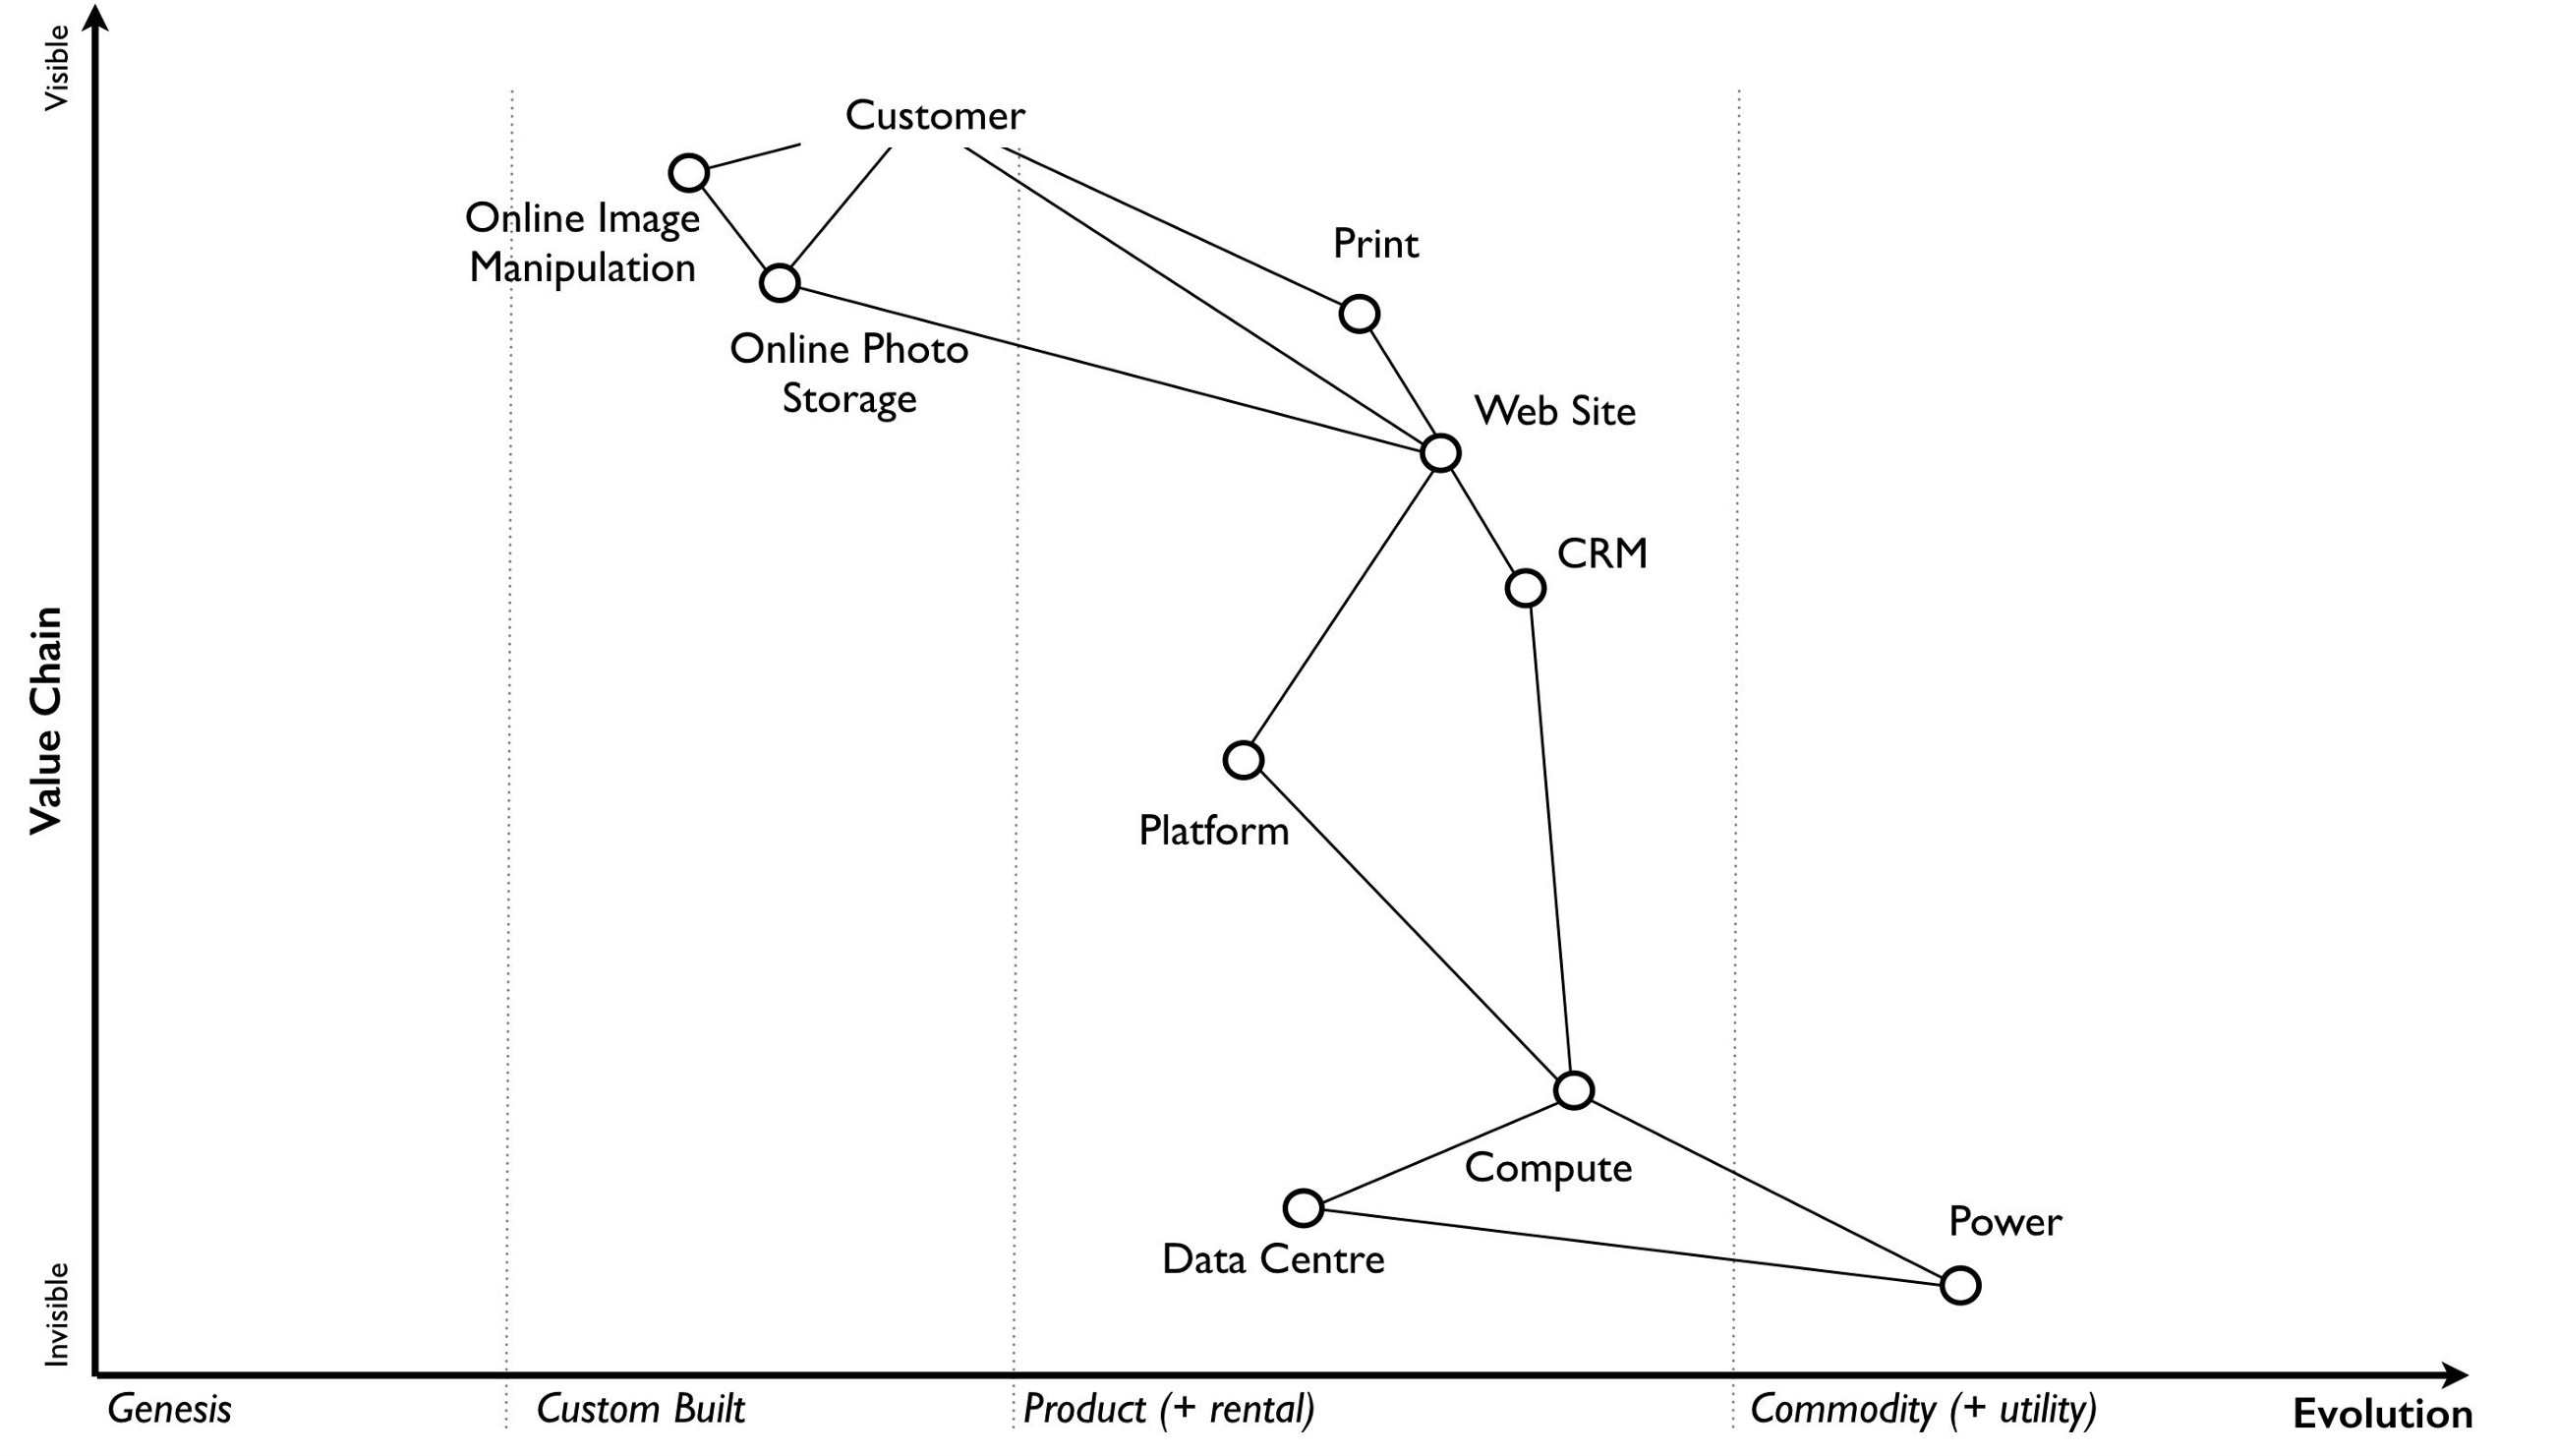
\includegraphics[width=435pt,height=320pt]{images/Fig8_original.jpeg}};
    
% \node[inner sep=0pt] (Fig8) at (5,5)
%     {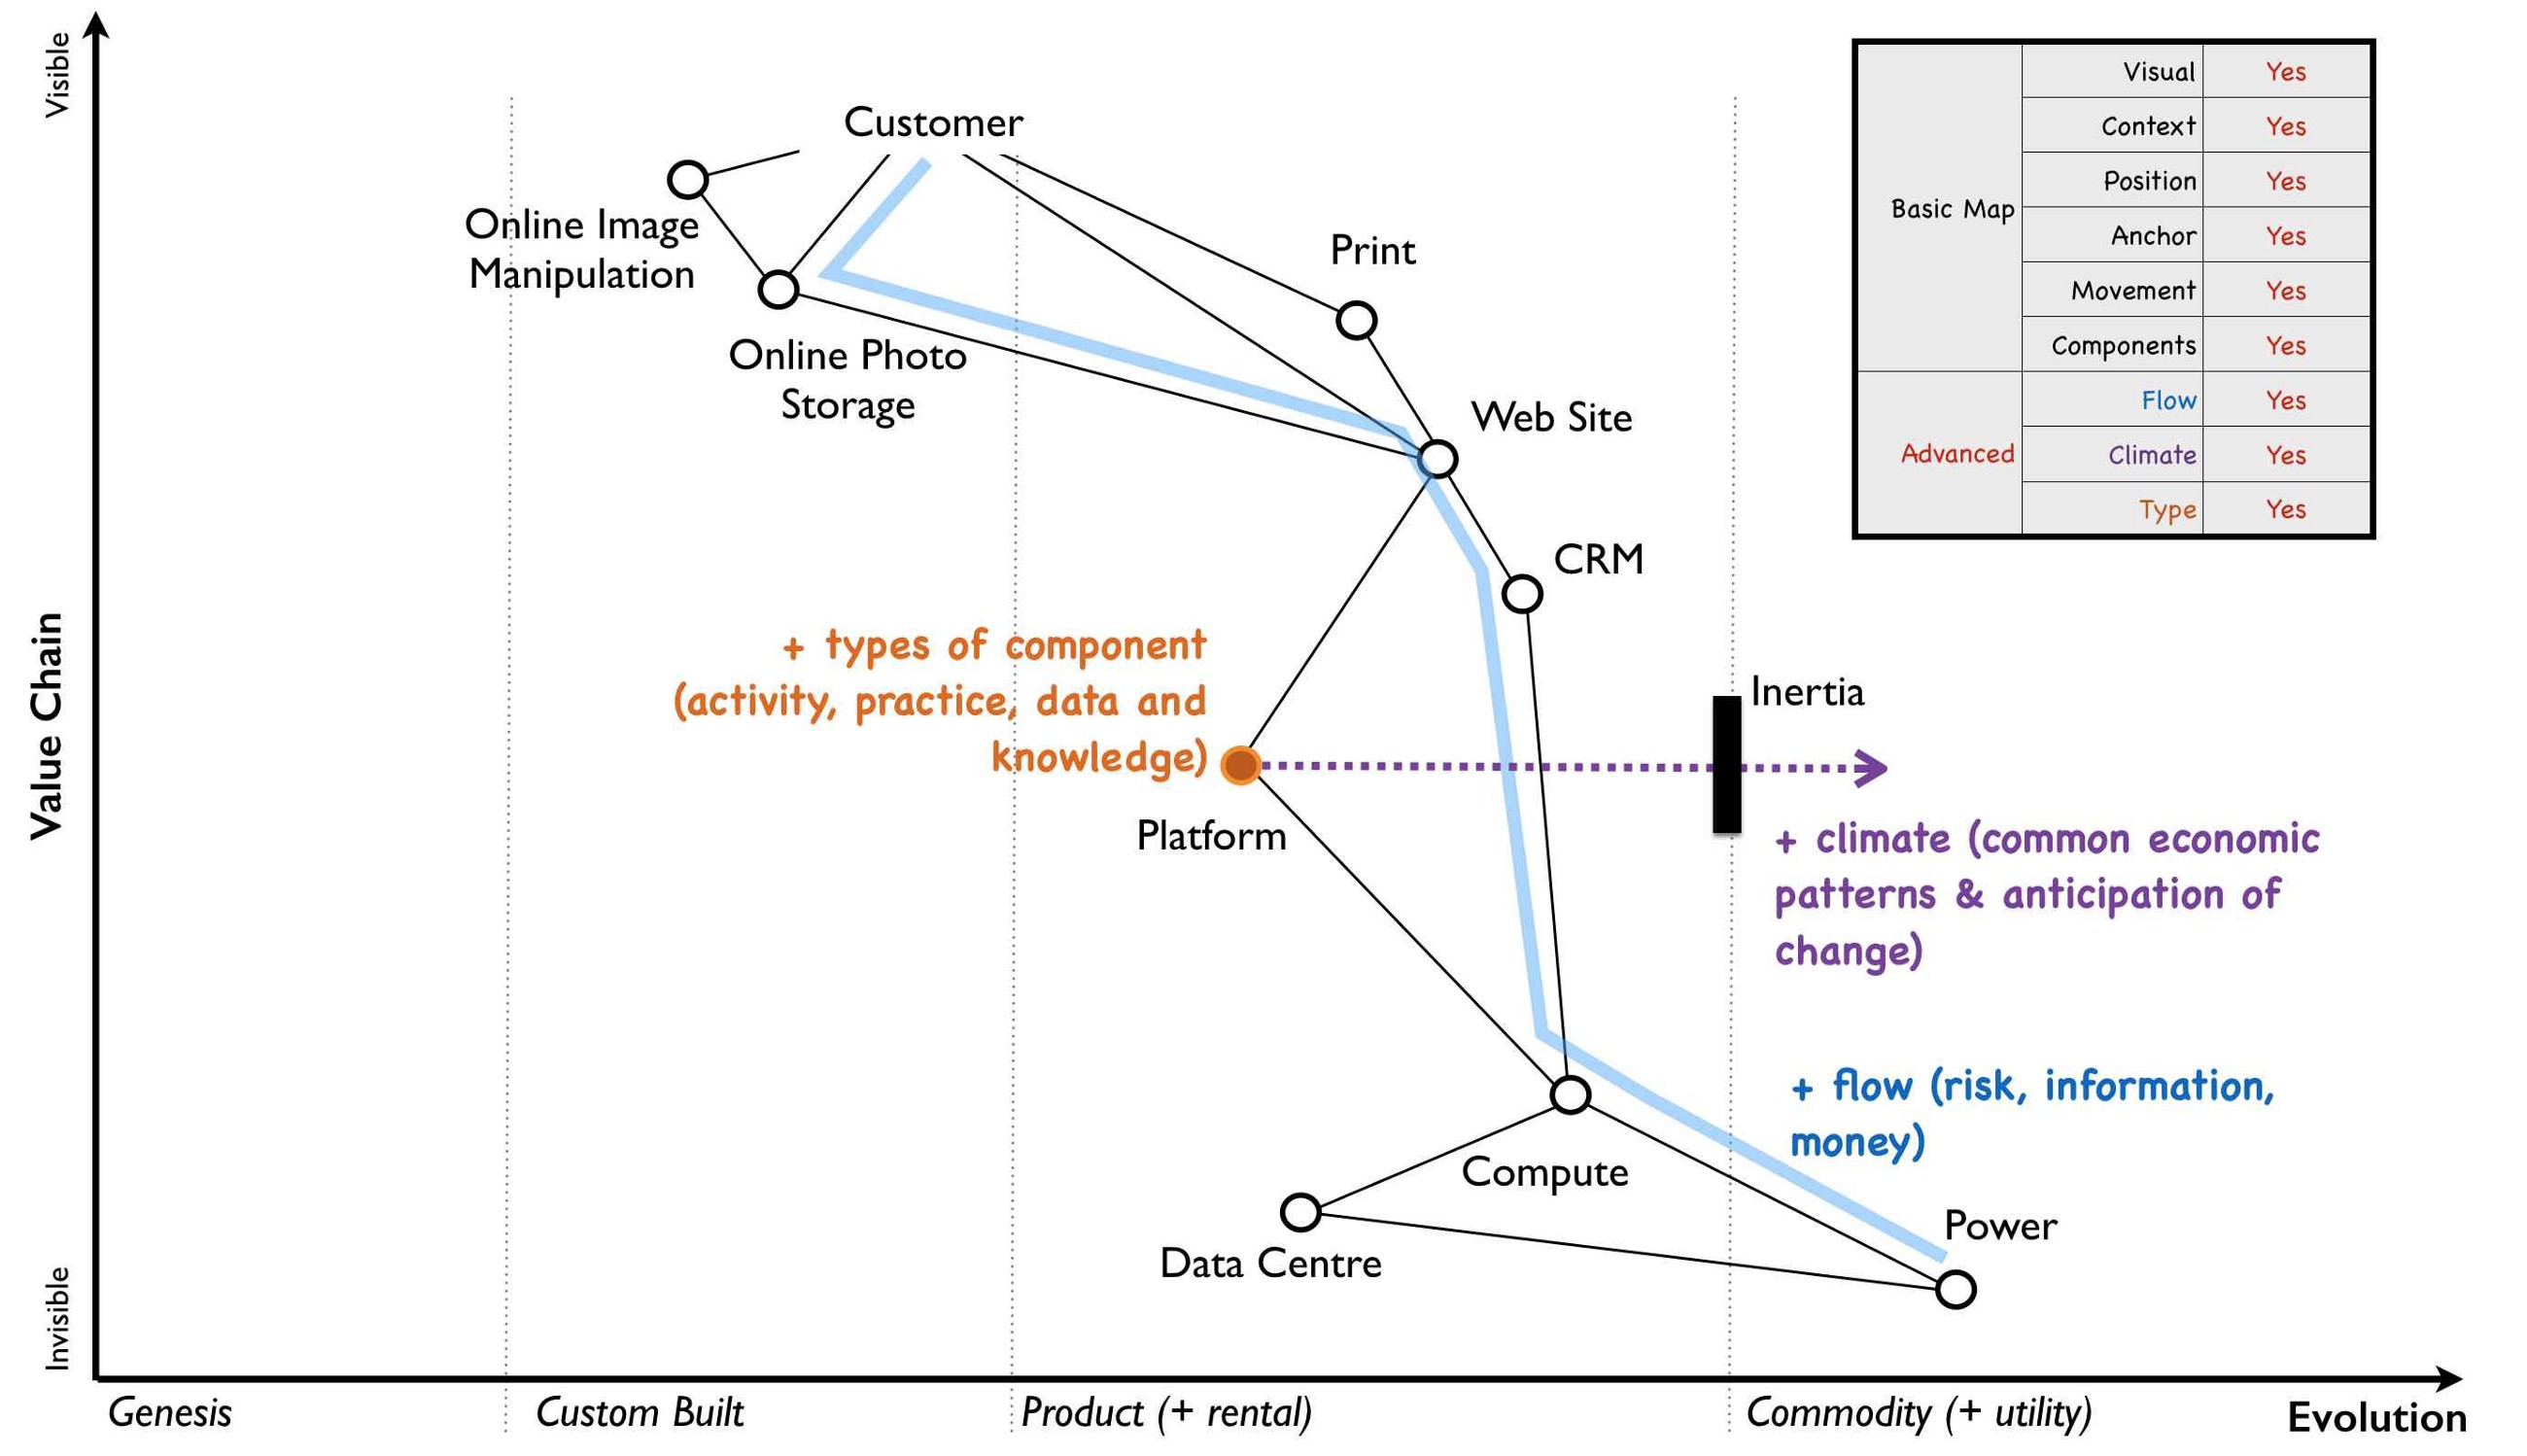
\includegraphics[width=435pt,height=320pt]{images/Fig11_original.jpeg}};
 
%Application Strata
%\fill[color=layer1,opacity=0.5] (0,7.5) rectangle (10,10);
%\node[align=left,rotate=90,color=black!] at (0.3,8.75) {\footnotesize{Applications}};

%Wardley maturity shading
\shade[left color=gray!80,right color=white,opacity=0.5] (0,0) rectangle (2,10);
\shade[left color=white,right color=white,opacity=0.5] (2,0) rectangle (8,10);
\shade[left color=white,right color=gray!80,opacity=0.5] (8,0) rectangle (10,10);


\end{pgfonlayer}